\documentclass[11pt,a4paper]{article}
\usepackage{amsmath,amssymb,amsthm}
\usepackage{graphicx}
\usepackage[margin=2.2cm]{geometry}
\usepackage{xcolor}
\usepackage{titlesec}
\usepackage{fancyhdr}
\usepackage{booktabs}
\usepackage{enumitem}
\usepackage{float}
\usepackage{hyperref}
\hypersetup{colorlinks=true,linkcolor=blue!70!black,urlcolor=blue!70!black}

\renewcommand{\topfraction}{0.9}
\renewcommand{\bottomfraction}{0.9}
\renewcommand{\textfraction}{0.07}
\renewcommand{\floatpagefraction}{0.7}
\setcounter{topnumber}{3}
\setcounter{bottomnumber}{3}
\setcounter{totalnumber}{5}

\definecolor{primary}{RGB}{0,51,102}
\definecolor{accent}{RGB}{204,102,0}

\titleformat{\section}{\Large\bfseries\color{primary}}{\thesection}{1em}{}
\titleformat{\subsection}{\large\bfseries\color{primary!80!black}}{\thesubsection}{1em}{}

\pagestyle{fancy}
\fancyhf{}
\fancyhead[L]{\small\color{primary}Essential Summary}
\fancyhead[R]{\small\color{primary}Li et al.\ (2016)}
\fancyfoot[C]{\thepage}
\renewcommand{\headrulewidth}{0.5pt}

\begin{document}

\begin{center}
{\LARGE\bfseries\color{primary}Essential Summary}\\[12pt]
{\large\bfseries Predicting Homoclinic and Heteroclinic Bifurcation\\of Generalized Duffing--Harmonic--van de Pol Oscillator}\\[8pt]
{\normalsize Zhenbo Li, Jiashi Tang, Ping Cai}\\[4pt]
{\small\itshape Qualitative Theory of Dynamical Systems, Vol.\ 15, No.\ 1, 19--37 (2016)\quad DOI: 10.1007/s12346-015-0138-z}\\[6pt]
{\small\rule{0.7\textwidth}{0.5pt}}\\[4pt]
{\small\color{accent}This is an author-prepared essential summary, not the original paper.\\Please cite the published version.}
\end{center}

\vspace{0.5em}

\section{Background and Motivation}

The Duffing--harmonic oscillator, characterized by a rational restoring force,
\begin{equation}
\ddot{x} + \frac{\lambda x + \delta x^3}{1 + \nu x^2} = 0
\label{eq:undamped}
\end{equation}
bridges two well-studied regimes: for small $x$, it behaves as a Duffing oscillator ($\ddot{x} + \delta x^3 \approx 0$); for large $x$, it approximates a linear harmonic oscillator ($\ddot{x} + (\delta/\nu) x \approx 0$). This dual nature makes it an excellent model for systems with amplitude-dependent stiffness transitions.

While the conservative Duffing--harmonic oscillator had been extensively studied via harmonic balance, homotopy analysis, and energy balance methods, the \textbf{damped} version---the generalized Duffing--harmonic--van de Pol oscillator---
\begin{equation}
\ddot{x} + \frac{\lambda x + \delta x^3}{1 + \nu x^2} = \varepsilon(\mu + \mu_1 x + \mu_2 x^2 + \mu_4 x^4)\dot{x}
\label{eq:damped}
\end{equation}
had received almost no attention. This paper fills that gap by applying the quadratic generalized harmonic function perturbation method to predict both homoclinic and heteroclinic bifurcations in this oscillator.

\section{Quadratic Generalized Harmonic Function}

\subsection{Solution Construction}

Building on the original GHFP method (JSV 2013), this paper constructs solutions in the form:
\begin{align}
x(t) &= a\sin^2\phi(t) + b \qquad \text{(homoclinic orbits)}\\
x(t) &= a\cos^2\phi(t) + b \qquad \text{(heteroclinic orbits)}
\label{eq:construction}
\end{align}

The nonlinear time transformation:
\begin{equation}
\frac{d\phi}{dt} = \Phi(\phi), \qquad \Phi(\phi + \pi) = \Phi(\phi)
\label{eq:NTT}
\end{equation}
maps the time domain to an angular domain where the solutions have a symmetric form.

\subsection{Homoclinic Orbits}

For a saddle point $H(h,0)$, the initial condition $c$ satisfies:
\begin{equation}
\int_h^c \frac{\lambda x + \delta x^3}{1 + \nu x^2} dx = 0
\label{eq:homoclinic_int}
\end{equation}
and the homoclinic solution must satisfy $x(\phi_{\pm\infty}) = h$. The angular velocity is obtained as:
\begin{equation}
\Phi(\phi) = \sqrt{\frac{2[V(b) - V(a\sin^2\phi + b)]}{(x'(\phi))^2}}
\label{eq:Phi_h}
\end{equation}
with $\Phi(0) = \Phi(\pi) = \sqrt{|g(h)/2a|} = 0$ ensuring infinite period at the saddle point.

\subsection{Heteroclinic Orbits}

For two distinct saddle points $H_1(h_1, 0)$ and $H_2(h_2, 0)$:
\begin{equation}
\lim_{t\to -\infty} x(t) = h_1, \qquad \lim_{t\to +\infty} x(t) = h_2
\label{eq:heteroclinic_limits}
\end{equation}
The constants $a$ and $b$ are determined by $\phi = 0 \to x = h_1$ and $\phi = \pi/2 \to x = h_2$. The angular velocity satisfies $\Phi(0) = \Phi(\pi/2) = 0$.

\section{Perturbation Procedure}

\subsection{Expansion and Key Assumption}

When $\varepsilon \neq 0$:
\begin{equation}
a = a_0 + \varepsilon a_1 + \cdots, \qquad \Phi = \Phi_0 + \varepsilon\Phi_1 + \cdots
\label{eq:expansion}
\end{equation}

The determining insight: \textbf{the $n$th-order approximate solution maintains the same functional form as the generating solution}:
\begin{align}
x_n &= a_n \sin^2\phi \quad \text{(homoclinic)}\\
x_n &= a_n \cos^2\phi \quad \text{(heteroclinic)}
\end{align}
This eliminates the cumbersome integrals that plague classical perturbation methods.

\subsection{Homoclinic Bifurcation Prediction}

The first-order consistency condition yields:
\begin{equation}
\boxed{\mu_c = -\frac{\int_0^\pi \Phi_0 (\mu_1 x_0 + \mu_2 x_0^2 + \mu_4 x_0^4)(\Phi_0 x_0') x_0' d\varphi}{\int_0^\pi \Phi_0^2 (x_0')^2 d\varphi}}
\label{eq:mu_c}
\end{equation}
This formula directly predicts the critical parameter value $\mu_c$ at which homoclinic bifurcation occurs.

\section{Key Results}

\subsection{Example 1: Duffing--Harmonic Oscillator with $(\mu_1, \mu_2, \mu_4)$ Damping}

For the system with $\lambda = \delta = \nu = 1$, the GHFP method accurately predicts homoclinic orbits across a wide range of $\varepsilon$ values.

\begin{figure}[htbp]
\centering
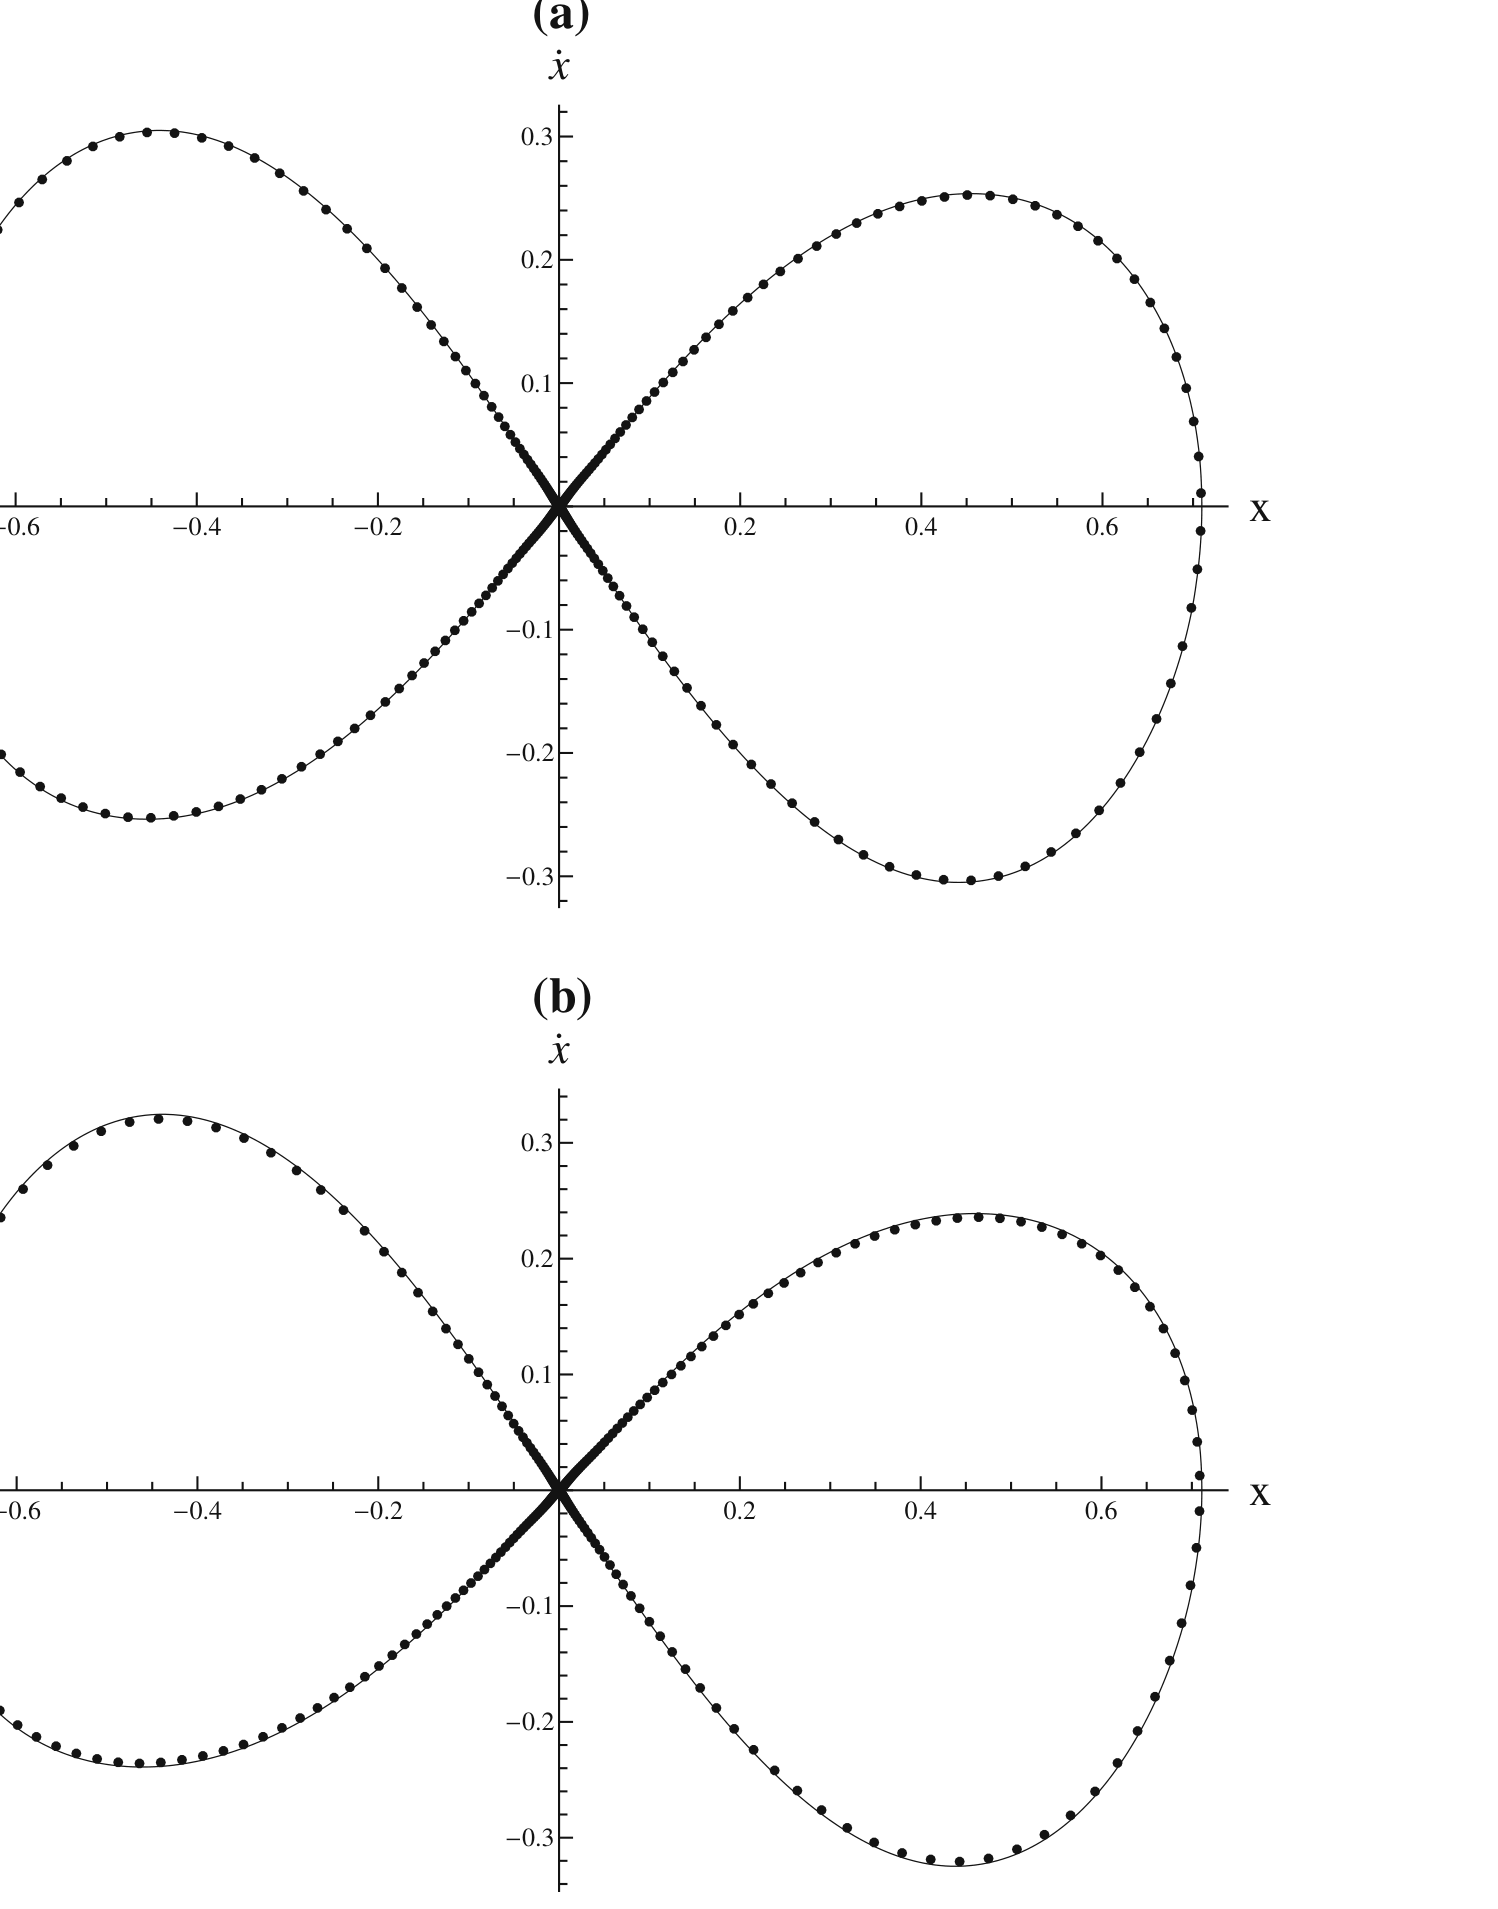
\includegraphics[width=\textwidth,height=0.42\textheight,keepaspectratio]{p6-fig1-homoclinic.png}
\caption{\textbf{Figure 1.} (Original Fig.\ 1) Homoclinic orbits for $\varepsilon=1.2, 2.0$. Solid lines: Runge--Kutta method. Dotted lines: GHFP method. Excellent agreement demonstrates the effectiveness of the quadratic generalized harmonic function approach for rational restoring forces.}
\end{figure}

\subsection{Example 2: Multiple Coexisting Homoclinic Orbits}

For a system with different parameters, the method captures two types of homoclinic orbits---one enclosing a single well and another enclosing both wells---at the same parameter values.

\begin{figure}[htbp]
\centering
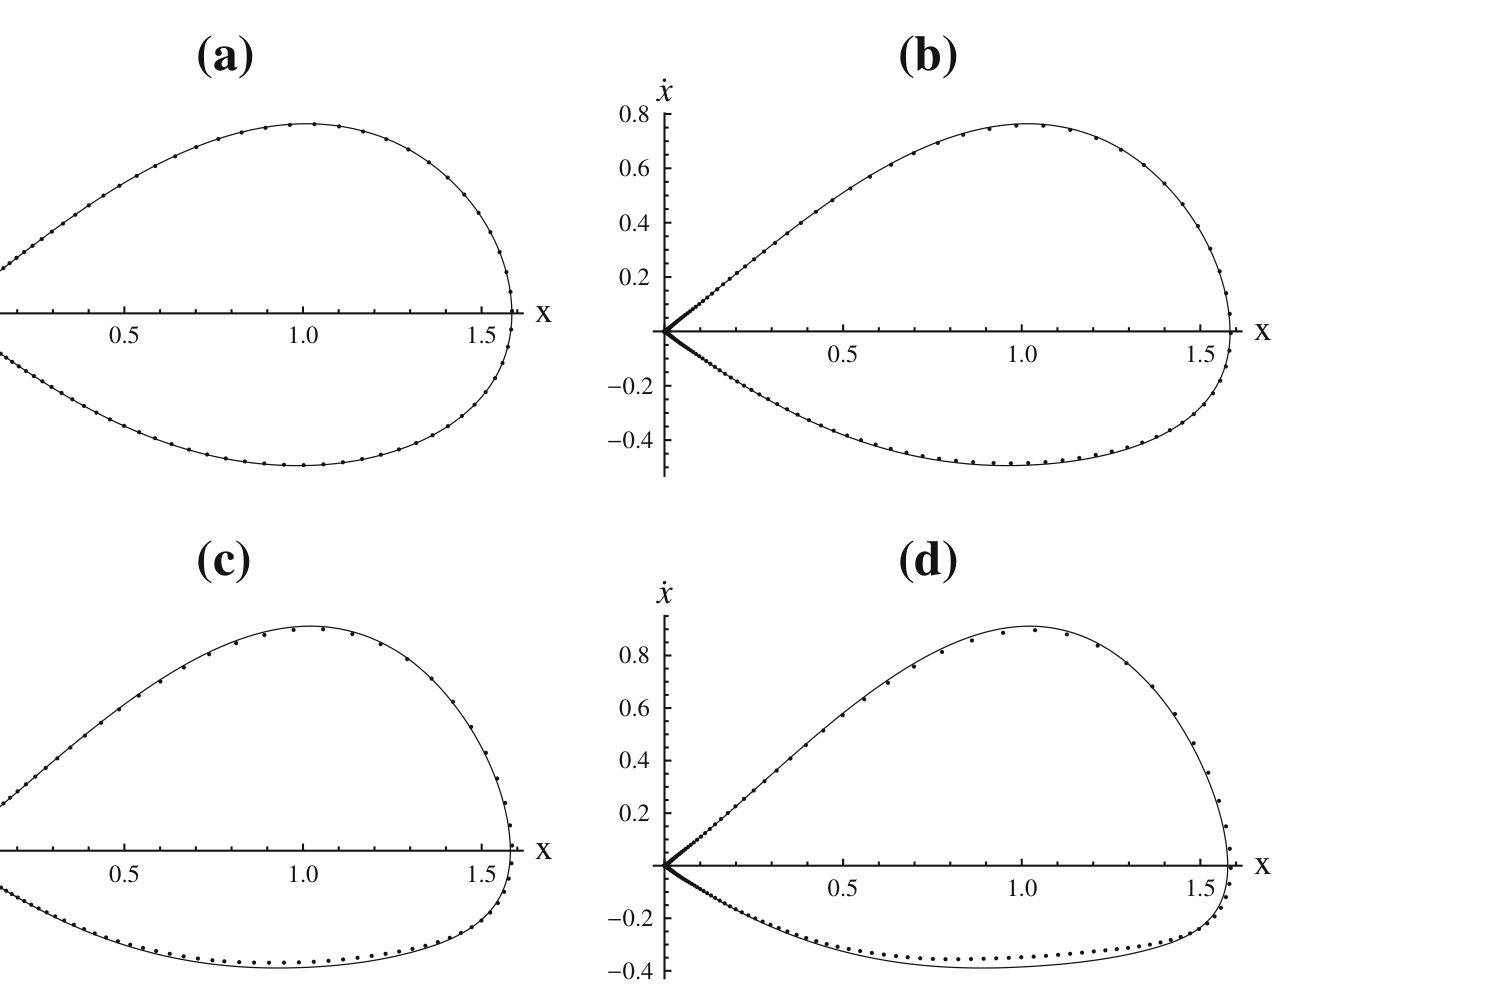
\includegraphics[width=\textwidth,height=0.40\textheight,keepaspectratio]{p6-fig2-homoclinic.png}
\caption{\textbf{Figure 2.} (Original Fig.\ 2) Homoclinic orbits for $\varepsilon=0.5, 1.0, 1.5, 2.0$. The method successfully tracks the orbits across a wide range, maintaining accuracy even at $\varepsilon=2.0$.}
\end{figure}

\subsection{Example 3: Heteroclinic Bifurcation Prediction}

For the heteroclinic case, the method predicts critical parameter values:
\begin{equation}
\mu_c = -0.1979871606 \quad (\varepsilon=0.5), \qquad \mu_c^{\text{(numerical)}} = -0.1977132821
\end{equation}
The relative error is approximately $0.14\%$.

\begin{figure}[htbp]
\centering
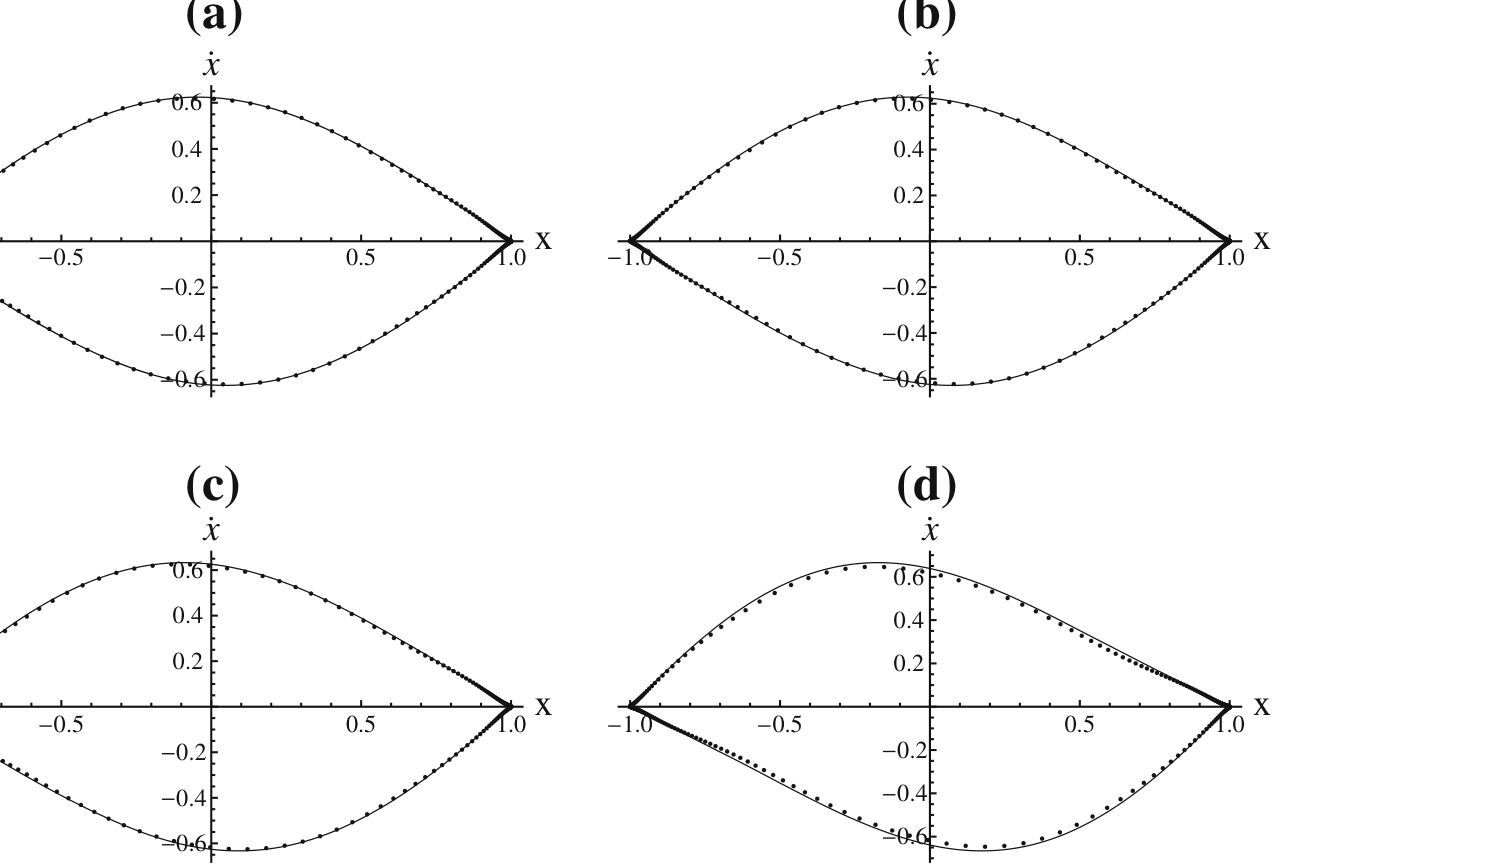
\includegraphics[width=0.85\textwidth,height=0.42\textheight,keepaspectratio]{p6-fig4-heteroclinic.png}
\caption{\textbf{Figure 3.} (Original Fig.\ 4) Heteroclinic orbits connecting two distinct saddle points for $\varepsilon=0.5, 0.8, 1.0, 2.0$. The method captures cross-saddle connections with remarkable accuracy.}
\end{figure}

\section{Significance}

\begin{enumerate}[leftmargin=2em]
\item \textbf{First application of GHFP to rational restoring forces:} Unlike the polynomial Helmholtz--Duffing oscillator (JSV 2013), the rational form $\frac{\lambda x + \delta x^3}{1+\nu x^2}$ introduces fundamentally different Fourier coefficient computations. The method's success here demonstrates its versatility.

\item \textbf{Simultaneous homoclinic and heteroclinic prediction:} The same framework handles both types of global bifurcations without modification---a capability not available with classical perturbation methods.

\item \textbf{Connection to the MGHFP series:} This paper bridges the original GHFP method (2013) and the modern MGHFP series (2024--2026), showing the evolution from polynomial to rational restoring forces.
\end{enumerate}

\section{Limitations}

\begin{itemize}[leftmargin=2em]
\item First-order perturbation limits accuracy when $\varepsilon > 2$ for some parameter regions.
\item The method requires analytical knowledge of the saddle points, which may become algebraically intractable for more complex restoring forces.
\item Only single-degree-of-freedom systems are considered.
\end{itemize}

\vfill
\begin{center}
\small\rule{0.5\textwidth}{0.3pt}\\[4pt]
\small\color{primary} Author: Zhenbo Li (lizhenbo@usc.edu.cn)\\
\small University of South China, School of Mathematics and Physics\\
\small Hunan Key Laboratory of Mathematical Modeling and Scientific Computing
\end{center}

\end{document}
